\documentclass[12pt, a4paper]{report}
\usepackage{styles}

\begin{document}
  \begin{titlepage}
  \begin{figure}
    
\includegraphics[width=0.5\linewidth]{logo_PXL_University_of_applied_sciences_and_arts.png}
  \end{figure}
  \vspace*{0.5cm}
  \begin{center}
    \Huge\textbf{\textcolor{pxlgreen}{Stageportfolio}}
  \end{center}
  \vspace{0.5cm}
  \begin{center}
    \LARGE\textbf{\textcolor{pxlgreen}{PXL-Digital}}
  \end{center}
  \vspace{2.5cm}
  \begin{center}
    \Large\textbf{Expertisecentrum PXL Smart ICT}
  \end{center}
  \vspace{3cm}
  \begin{tabularx}{\linewidth}{l l}
    Student: & \textbf{Vic Segers}\\
    Bedrijfspromotor: & \textbf{Tim Dupont}\\
    Hogeschoolpromotor: & \textbf{Tim Dupont}
  \end{tabularx}
  \vfill
  \framebox{%
    \begin{minipage}{0.3\linewidth}
      Hogeschool PXL\\
      Elfde Liniestraat 24\\
      B-3500 Hasselt
      \bigbreak
      \href{https://www.pxl.be/}{www.pxl.be}
    \end{minipage}}
\end{titlepage}
  \blankpage
  \begin{titlepage}
  \begin{figure}
    
\includegraphics[width=0.5\linewidth]{logo_PXL_University_of_applied_sciences_and_arts.png}
  \end{figure}
  \vspace*{0.5cm}
  \begin{center}
    \Huge\textbf{\textcolor{pxlgreen}{Stageportfolio}}
  \end{center}
  \vspace{0.5cm}
  \begin{center}
    \LARGE\textbf{\textcolor{pxlgreen}{PXL-Digital}}
  \end{center}
  \vspace{2.5cm}
  \begin{center}
    \Large\textbf{Expertisecentrum PXL Smart ICT}
  \end{center}
  \vspace{3cm}
  \begin{tabularx}{\linewidth}{l l}
    Student: & \textbf{Vic Segers}\\
    Bedrijfspromotor: & \textbf{Tim Dupont}\\
    Hogeschoolpromotor: & \textbf{Tim Dupont}
  \end{tabularx}
  \vfill
  \framebox{%
    \begin{minipage}{0.3\linewidth}
      Hogeschool PXL\\
      Elfde Liniestraat 24\\
      B-3500 Hasselt
      \bigbreak
      \href{https://www.pxl.be/}{www.pxl.be}
    \end{minipage}}
\end{titlepage}
  \pagestyle{plain}
  \pagenumbering{roman}
  \nonumchapter{Acknowledgements}
  Foremost, I would like to express my sincere gratitude ot my promotor Tim Dupont for the continuous support and feedback throughout the internship. Besides my promotor, I would like to thank all employees of Smart ICT for making this internship possible and for their guidance.

I am ever so grateful for this oppertunity given to me by PXL University of Applied Sciences and Arts and Smart ICT. Many of my skills are improved during these twelve weeks. Aswell as I have gotten a taste of a real work environment. During this whole internship, the communication from PXL University and Smart ICT was flawless. Even during the COVID\hyp{}19 period, all guideliness and measurements concerning the virus were clearly and rapidly informed to everyone.

At last, I give thanks to my fellow interns at Smart ICT that assisted me during my internship: Bavo Knaeps and Borcherd van Brakell van Wadenoyen en Doorwerth. If it were not for them, this internship would not have turned out as great as it did.
  \nonumchapter{Abstract}
  The center of expertise PXL Smart ICT, part of the PXL University of Applied Sciences and Arts research department, has an ongoing project for enabling IT companies to implement \ac{uav} projects via rapid robot prototyping. This internship is an integral part of that research project.

One of the goals of this internship project is updating and fine\hyp{}tuning an existing Smart \acs{uav} software architecture. Another objective is researching the realm of \ac{slam} algorithms. Robots utilize these algorithms to create a map using their sensors and at the same time locate themselves within this map. Once a map of a certain area exists, a path planning method can be executed in order to navigate between points. Previous goals and objectives will be combined into a showcase where a \acs{uav} makes use of a SLAM method to fly and navigate autonomously in a previously unknown dynamic environment.

A \acs{slam} algorithm behaves the same way a human being would when dropped in an unknown environment. A human being opens their eyes and looks around in search of reference points in their environment. These reference points are used as landmarks for their localization. However, unlike humans who use their senses, a \acs{uav} uses sensors to get information about its surroundings and uses this to search for reference points. While flying, it can estimate its position based on the movement of these landmarks.

The internship project uses a combination of diverse technologies. Python is predominately used as the programming language. Between the different hardware components and the controlling software, \acs{ros} is being used. ROS is an open\hyp{}source robotics middleware. Remote controlling the \acs{uav} is done by using MAVROS. The controlling software implemented with Python and ROS uses MAVROS to communicate via the \acs{mavlink} protocol. \acs{mavlink} is a lightweight messaging protocol for communicating with \acsp{uav} and between onboard \acs{uav} components. An autopilot receives these commands and translates them to actual actions that the \acs{uav} has to execute. All autopilots used during the internship are based on the open\hyp{}source PX4 flight control software for \acsp{uav} and other unmanned vehicles. For safety and testing purposes, the entire internship project is developed in an open\hyp{}source \acs{3d} robotics simulator, Gazebo. To make the system flexible, modular, and consistent a multi\hyp{}container Docker environment is used.
  \clearpage
  \phantomsection
  \addcontentsline{toc}{chapter}{Table of Contents}
  \tableofcontents
  \clearpage
  \phantomsection
  \addcontentsline{toc}{chapter}{List of Figures}
  \listoffigures
  \clearpage
  \phantomsection
  \addcontentsline{toc}{chapter}{List of Tables}
  \listoftables
  \nonumchapter{List of Abbreviations}
  \begin{acronym}[RTAB-Map]
  \acro{1d}[1D]{One Dimensional}
  \acro{2d}[2D]{Two Dimensional}
  \acro{2.5d}[2.5D]{Two\hyp{}and\hyp{}a\hyp{}half Dimensional}
  \acro{3d}[3D]{Three Dimensional}
  \acro{ai}[AI]{Artificial Intelligence}
  \acro{ar}[AR]{Augmentend Reality}
  \acro{bair}[BAIR]{Berkeley Artificial Intelligence Research}
  \acro{blam}[BLAM!]{Berkeley Localization And Mapping}
  \acro{crc}[CRC]{Cyclic Redundancy Check}
  \acro{gps}[GPS]{Global Positioning System}
  \acro{gtsam}[GTSAM]{Georgia Tech Smoothing And Mapping}
  \acro{gui}[GUI]{Graphical User Interface}
  \acro{lidar}[LiDAR]{Light Detection And Ranging}
  \acro{ict}[ICT]{Information Communications Technology}
  \acro{imu}[IMU]{Inertial Mesurement Unit}
  \acro{iot}[IoT]{Internet of Things}
  \acro{mavlink}[MAVLink]{Micro Air Vehicle Link}
  \acro{opengl}[OpenGL]{Open Graphics Library}
  \acro{qrcode}[QR code]{Quick Response code}
  \acro{ros}[ROS]{Robotic Operating System}
  \acro{rgbd}[RGB\hyp{}D]{Red Green Blue Depth}
  \acro{slam}[SLAM]{Simultaneous Localization And Mapping}
  \acro{stx}[STX]{start\hyp{}of\hyp{}text}
  \acro{rtabmap}[RTAB\hyp{}Map]{Real\hyp{}Time Appearance\hyp{}Based Mapping}
  \acro{uav}[UAV]{Unmanned Aerial Vehicle}
  \acro{vm}[VM]{Virtual Machine}
  \acro{vr}[VR]{Virtual Reality}
\end{acronym}
  \clearpage
  \pagenumbering{arabic}
  \nonumchapter{Introduction}
  In an era where \acsp{uav} are becoming more advanced, cheaper, and more socially accepted, they can perform tasks no one would have thought a few years ago. What if these tasks could be executed without human interference? Currently, cars are on the verge of driving fully autonomous. Then would it not be possible for \acsp{uav} to fly autonomously as well?

This paper will focus on the autonomous navigation of a \acs{uav} in an indoor dynamic environment. Some practical applications could be the complete \acs{3d} mapping of a building's inside, an inspection of huge shopping malls, and photography of large indoor constructions. \cite{spiral_robotics}

To promote the development of \acs{uav} applications, an architecture for their development is created. This architecture is a multi\hyp{}container Docker system, with Gazebo as the simulator of \acsp{uav} and the environment, and \acs{ros} to combine all used technologies. This project, with the architecture as a backbone, has a showcase where the conducted research is demonstrated.

  \chapter{Traineeship report}
    \section{About the company}
    The center of expertise Smart \acs{ict} of Hogeschool PXL consists of 21 all\hyp{}round employees and bundles their knowledge of \acs{ict} (software, project management, software architecture, systems) and electronics (focus on hardware and embedded software). The link with education is ensured via the new department PXL\hyp{}Digital, which besides the bachelor programs applied informatics and electronics\hyp{}\acs{ict} also represents graduate programs \acl{iot}, Programming, and Systems \& Networks, with about 1500 students in total.

Smart \acs{ict} is pursuing a double course: on the one hand, efforts are being made in many vertical domains, such as \acs{vr}/\acs{ar}, \ac{iot}, Blockchain, and \acl{ai} \& Robotics; on the other hand, horizontal support is offered to other centers of expertise, through the development of mobile or web\hyp{}based applications. Smart \acs{ict} offers support to partners from various sectors by responding to practical questions about \acs{ict} advice for companies, organizations, and smart cities. The three areas in which Smart \acs{ict} is a priority are \acs{vr} and \acs{ar}, \acl{iot} and \acl{ai} \& Robotics. Finally, Smart \acs{ict} has set itself the goal of evaluating the use of new technologies and transferring these insights to specific target groups, such as the construction sector, education, the retail sector, or the healthcare sector.

I chose Smart \acs{ict} because of my interest in \acl{ai} \& Robotics. It also allowed me to continue working on a project I initiated during my bachelor program. Smart \acs{ict} is an expertise center where research is central, which I consciously chose for transferring to a master's program.
    \clearpage
    \section{Technologies}
    This section provides a brief description of all the technologies that are used throughout the project. It also provides an explanation of why the chosen technologies are used in this project. How these technologies are connected and their communication are visualized and described in the implementation section.
      \subsection{ROS}
      \ac{ros} is an open\hyp{}source, meta\hyp{}operating system for robots. A meta\hyp{}operating system provides services expected from an operating system, including hardware abstraction, low\hyp{}level device control, implementation of commonly\hyp{}used functionality, message\hyp{}passing between processes, and package management. \acs{ros} also provides tools and libraries for obtaining, building, writing, and running code across multiple computers. \cite{ros_introduction}

The primary goal of \acs{ros} is to support code reuse in robotics research and development. \acs{ros} is a distributed framework of processes - also called nodes - that enables executables to be individually designed and loosely coupled at runtime. By grouping these processes, packages are formed. These packages can be easily shared and distributed. By supporting a federated system of code repositories, \acs{ros} enables the distribution of collaboration. This design enables independent decisions about development and implementation, but can be brought together with the \acs{ros} infrastructure tools. \cite{newman2017systematic}

The nodes of \acs{ros} communicate with each other by publishing messages to topics. A message is a simple data structure, consisting of typed fields. The standard primitive types (integer, floating\hyp{}point, strings, etc.) are supported in these messages, as are arrays of the primitive types. \acs{ros} allows custom defined messages to be sent over its network. Other nodes can subscribe to topics and receive all messages sent to those topics. When a message is received, a callback is triggered that handles the message or acts on something. The \acs{ros} Master node provides names and registration services for the rest of the nodes in the system. This is how a single node can find another. \cite{ros_messages}

In this project, \acs{ros} is used as a communication medium. It allows the chosen technologies to talk with another in a reliable and standardized manner. \acs{ros} can be considered as the glue that combines the different technologies and creates a whole.
      \subsection{Gazebo}
      Gazebo is an open-source \acs{3d} dynamic simulator. It can simulate populations of robots in complex environments with high accuracy and efficiency. Gazebo is similar to game engines, but with a much higher degree of fidelity. Sensors simulated in this environment use this fidelity to function almost in the same way as they would in the real world. \cite{gazebo_beginner_overview} \cite{ackerman2016gazebo}

Gazebo is able to connect with \acs{ros} and be used as a replacement of the real world. The connection with \acs{ros} is realized through a set of \acs{ros} packages named \textit{gazebo\_ros\_pkgs}.
This set contains a package that stores all messages and service data structures needed for interacting with Gazebo. Another package provides robot\hyp{}independent Gazebo plugins for sensors, motors, and dynamic components. The set also has a package that allows for interfacing Gazebo with \acs{ros}. \cite{gazebo_ros_overview} \cite{gazebo_ros_control}

Gazebo is the standard for simulation when developing \acs{ros} projects because of its great compatibility with \acs{ros}. That is why Gazebo is chosen for this project. The main reasons for developing in a simulation are safety, consistency, economic, and testing purposes. A \acs{uav} can be a dangerous and expensive machine. If something went wrong during testing, the \acs{uav} could be damaged, or even worse a human could get hurt. That is why Gazebo is a great option for rapid robot prototyping.

\begin{figure}[!h]
  \centering
  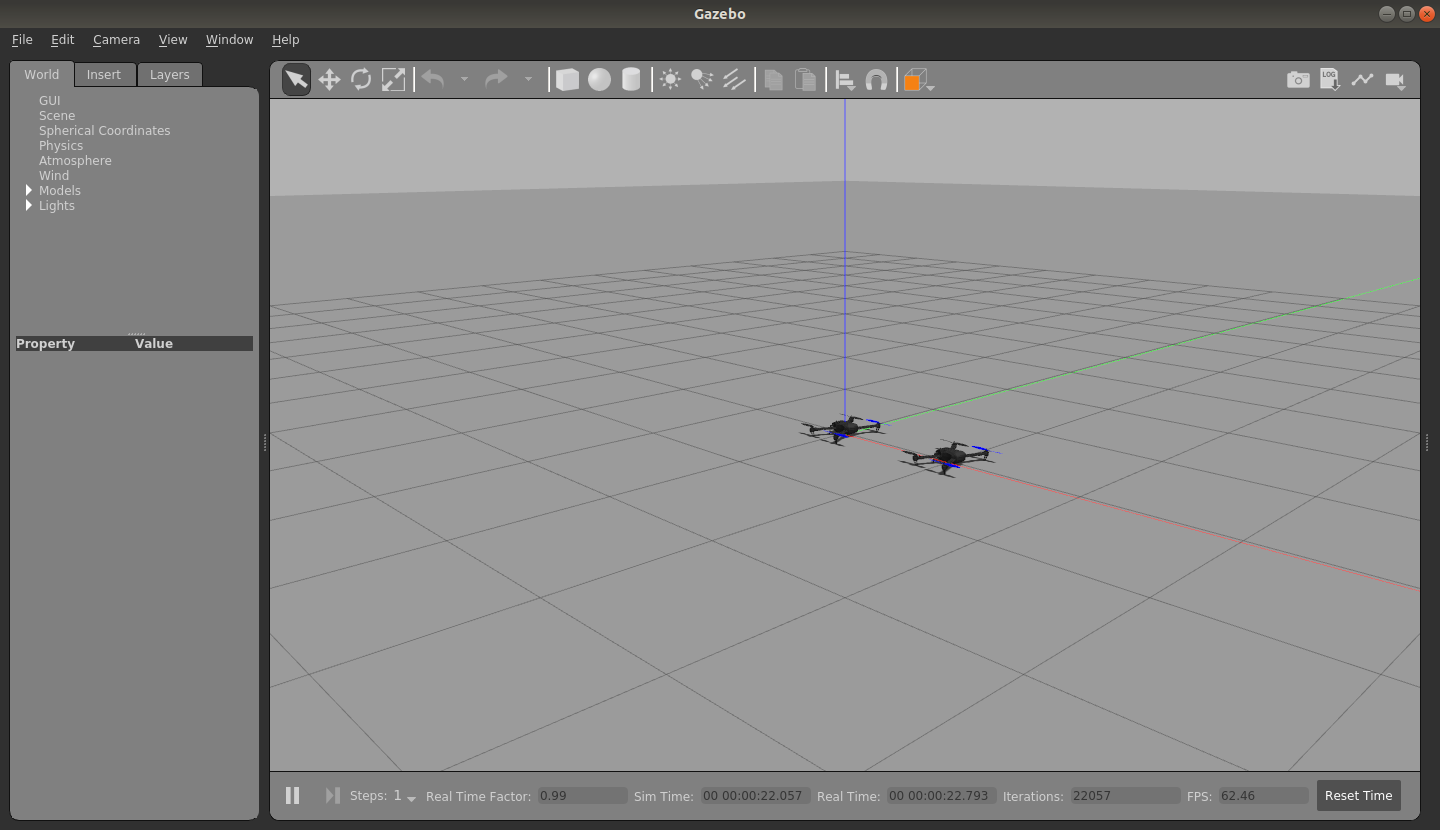
\includegraphics[width=\linewidth]{images/gazebo.png}
  \caption{Gazebo simulation}
\end{figure}
      \subsection{MAVROS}
      % https://mavlink.io/en/
MAVROS is an open\hyp{}source translation layer between \acs{ros} and \acs{mavlink}. \acs{mavlink} is a lightweight messaging protocol for communicating with unmanned vehicles. The key features of \acs{mavlink} are its efficiency, reliability, support of many programming languages, capability up to 255 concurrent systems on the network, and ability to enable offboard and onboard communications. \acs{mavlink} 1 has just eight bytes overhead per packet and \acs{mavlink} 2 has fourteen to increase its security. Therefore this protocol is very well suited for applications with very limited communication bandwidth. \cite{mavlink_developer_guide}

In this project, MAVROS is used for communication between the written code and the drone. MAVROS allows for coding on a higher abstraction, with the use of its library.
      \subsection{PX4 Autopilot}
      % https://px4.io/
% https://www.dronecode.org/projects/
The PX4 Autopilot is an open\hyp{}source autopilot system designed for low\hyp{}cost \acsp{uav}. The autopilot presents the current de-facto standard in the drone industry and is the leading research platform for drones. On top of that, it also has some successful applications for underwater vehicles and boats. The PX4 Autopilot provides guidance, navigation, control algorithms, and estimators for attitude and position. Thanks to its more flexible hardware and software, modifications are allowed to satisfy special requirements. \cite{px4} \cite{dronecode_projects}

% ~/Desktop/FM-ImplementationofanAutonomousNavigationAlgorithmwithCollisionAvoidanceforanUAV2018.pdf
Because the software is supported in multiple simulation choices, such as Gazebo. The PX4 Autopilot uses \acs{mavlink} as a communication tool. Therefore it can be controlled by \acs{ros}. The build\hyp{}in mode \textit{OFFBOARD} provides full control of the vehicle. \cite{mimmoimplementation}

The PX4 software also provides a model of a 3DR Iris Quadrotor that is compatible with Gazebo. The Iris is the default fixed\hyp{}wing drone of PX4. The type of drone is not important when simulating, therefore the default is kept.
      \subsection{Python}
      Python is a high\hyp{}level general\hyp{}purpose programming language, created by Guido van Rossum. It is developed as an interpreted language, the code is automatically compiled to byte code and executed. Python's philosophy emphasizes code readability achieved by its use of significant whitespace. Mostly Python is not used for its speed or performance because several studies have shown that it is slower than widely\hyp{}used programming languages, such as Java and C++. However, Python has the option to be extended in C and C++ to speed it up and even be used for compute\hyp{}intensive tasks. Its strong structuring constructs and its consistent use of objects enables programmers to write clear and logical applications. \cite{kuhlman2009python}

\acs{ros} is mainly developed using two languages, C++ and Python. For this project Python was the obvious choice because of its simplicity and readability. The used packages are written in C++ for performance.
      \clearpage
      \subsection{Docker}
      % https://opensource.com/resources/what-docker
Docker is an open\hyp{}source tool designed to simplify the creation, deployment, and running process of applications through the usage of containers. Containers allow the packaging of an application with all of the parts it needs, such as libraries and other dependencies. The application will run on any Linux machine regardless of any customized settings of that machine, because of the isolation of these containers. \cite{opensource_what_is_docker}

% https://opensource.com/resources/what-docker
Often the comparison is made with a virtual machine. But unlike a virtual machine, Docker does not need virtualization of a whole operating system. The applications run by Docker use the same Linux kernel as the host system. Therefore, compared to a virtual machine, it has a significant reduction in size and a boost in performance. \cite{opensource_what_is_docker}

% https://docs.docker.com/get-started/overview/
Running Docker containers requires images. An image is a read\hyp{}only template with commands for creating a container. These images can be obtained by two methods: creating your own or pulling from a registry. Pulling an image from a registry is the equivalent of downloading from the internet, these images are premade. Building your image requires a Dockerfile, in this file a set of Docker commands are defined that define the image. A container is a runnable instance of an image. This container can be started, stopped, moved, or deleted. After modifying the container, it can be saved back to an image for later use. The image can then be pushed back to the registry. \cite{docker_get_started_overview}

This project mainly uses Docker for an isolation option lighter than a virtual machine, its consistency, and scalability. However, the increased freedom is also a bonus. Knowing there is always a stable backup no matter which software or packages you experiment with.
      \subsection{RViz}
      RViz is a three\hyp{}dimensional visualization tool for \acs{ros} applications. It can provide a view of the robot model and the captured sensor information. RViz can display data from sensors like cameras and lasers in a \acs{2d} or \acs{3d} environment. In order to get the data sent through \acs{ros}, it has to be launched as a node so it can listen to all topics needed. \cite{aws_robomaker_developer_guide}

This project uses RViz to visually test the written and implemented code. It allows playback of previously saved missions and visualizing all captured points throughout that mission. RViz can function as a replacement for Gazebo's visuals when Gazebo is running headless to increase performance.
      \clearpage
    \section{Implementation}
    This section describes why these technologies are implemented in this project and how they interact with each other. It also explains the reasoning behind the two large components that this project contains. Those are the architecture and the showcase. The architecture is a clean environment made for developing \acs{uav} applications. The showcase in the implementation of the research topic with the architecture as a base.

All elements of the project are built in Docker containers. This allows for a consistent and clean environment for development. As well as a more robust and realistic system. In a real\hyp{}life scenario, not all components are in direct contact with another. For example, the onboard controller of one \acs{uav} does not share files with the onboard controller of another. This multi\hyp{}container environment communicates through a Docker network.
      \subsection{Architecture}
      The architecture consists of three containers being a controller, keyboard teleoperation, and a simulator. The simulator runs a Gazebo world that supports multiple 3DR Iris Quadrotor \acsp{uav} with each a PX4 Autopilot. The controller sends MAVROS commands to the \acsp{uav} for arming and changing their mode to \textit{OFFBOARD}. The \textit{OFFBOARD} mode provides full control of the \acsp{uav} through Python code. In the keyboard teleoperation container, pressed keys are parsed to the controller where they are translated to commands and send to the \acsp{uav}.

The containers in the architecture are run from different images. The simulation image has an \acs{opengl} base image or a specific NVIDIA base image if the host computer has NVIDIA installed. Adding to this base image, the simulation has \acs{ros} Melodic, MAVROS, Gazebo 9, the PX4 Firmware and their dependencies installed. There are two other images used in this project, a \acs{ros} base image and a MAVROS image. The keyboard teleoperation container uses the \acs{ros} base image with only \acs{ros} Melodic installed. The controller needs MAVROS to send commands to the \acsp{uav} and therefore uses the MAVROS image that extends from the \acs{ros} base image with the installation of MAVROS.

The goal of the architecture is to enable developers to develop drone applications without having to create a workspace or installing software manually. The repository contains scripts to automate all commands to build, run and stop the containers necessary for the development. The architecture supports drone and multi-drone applications.
      \clearpage
      \subsection{Showcase}
      The showcase uses the architecture as a base and adds features referencing the research topic. The simulation image of the architecture is used as a base for the one in the showcase. Three more images are added for containers that run a \acs{slam} algorithm, a path planning algorithm, and a \acs{qrcode} detector. These algorithms and the detector are clarified in the chapter of the research topic.

\begin{figure}[!h]
  \centering
  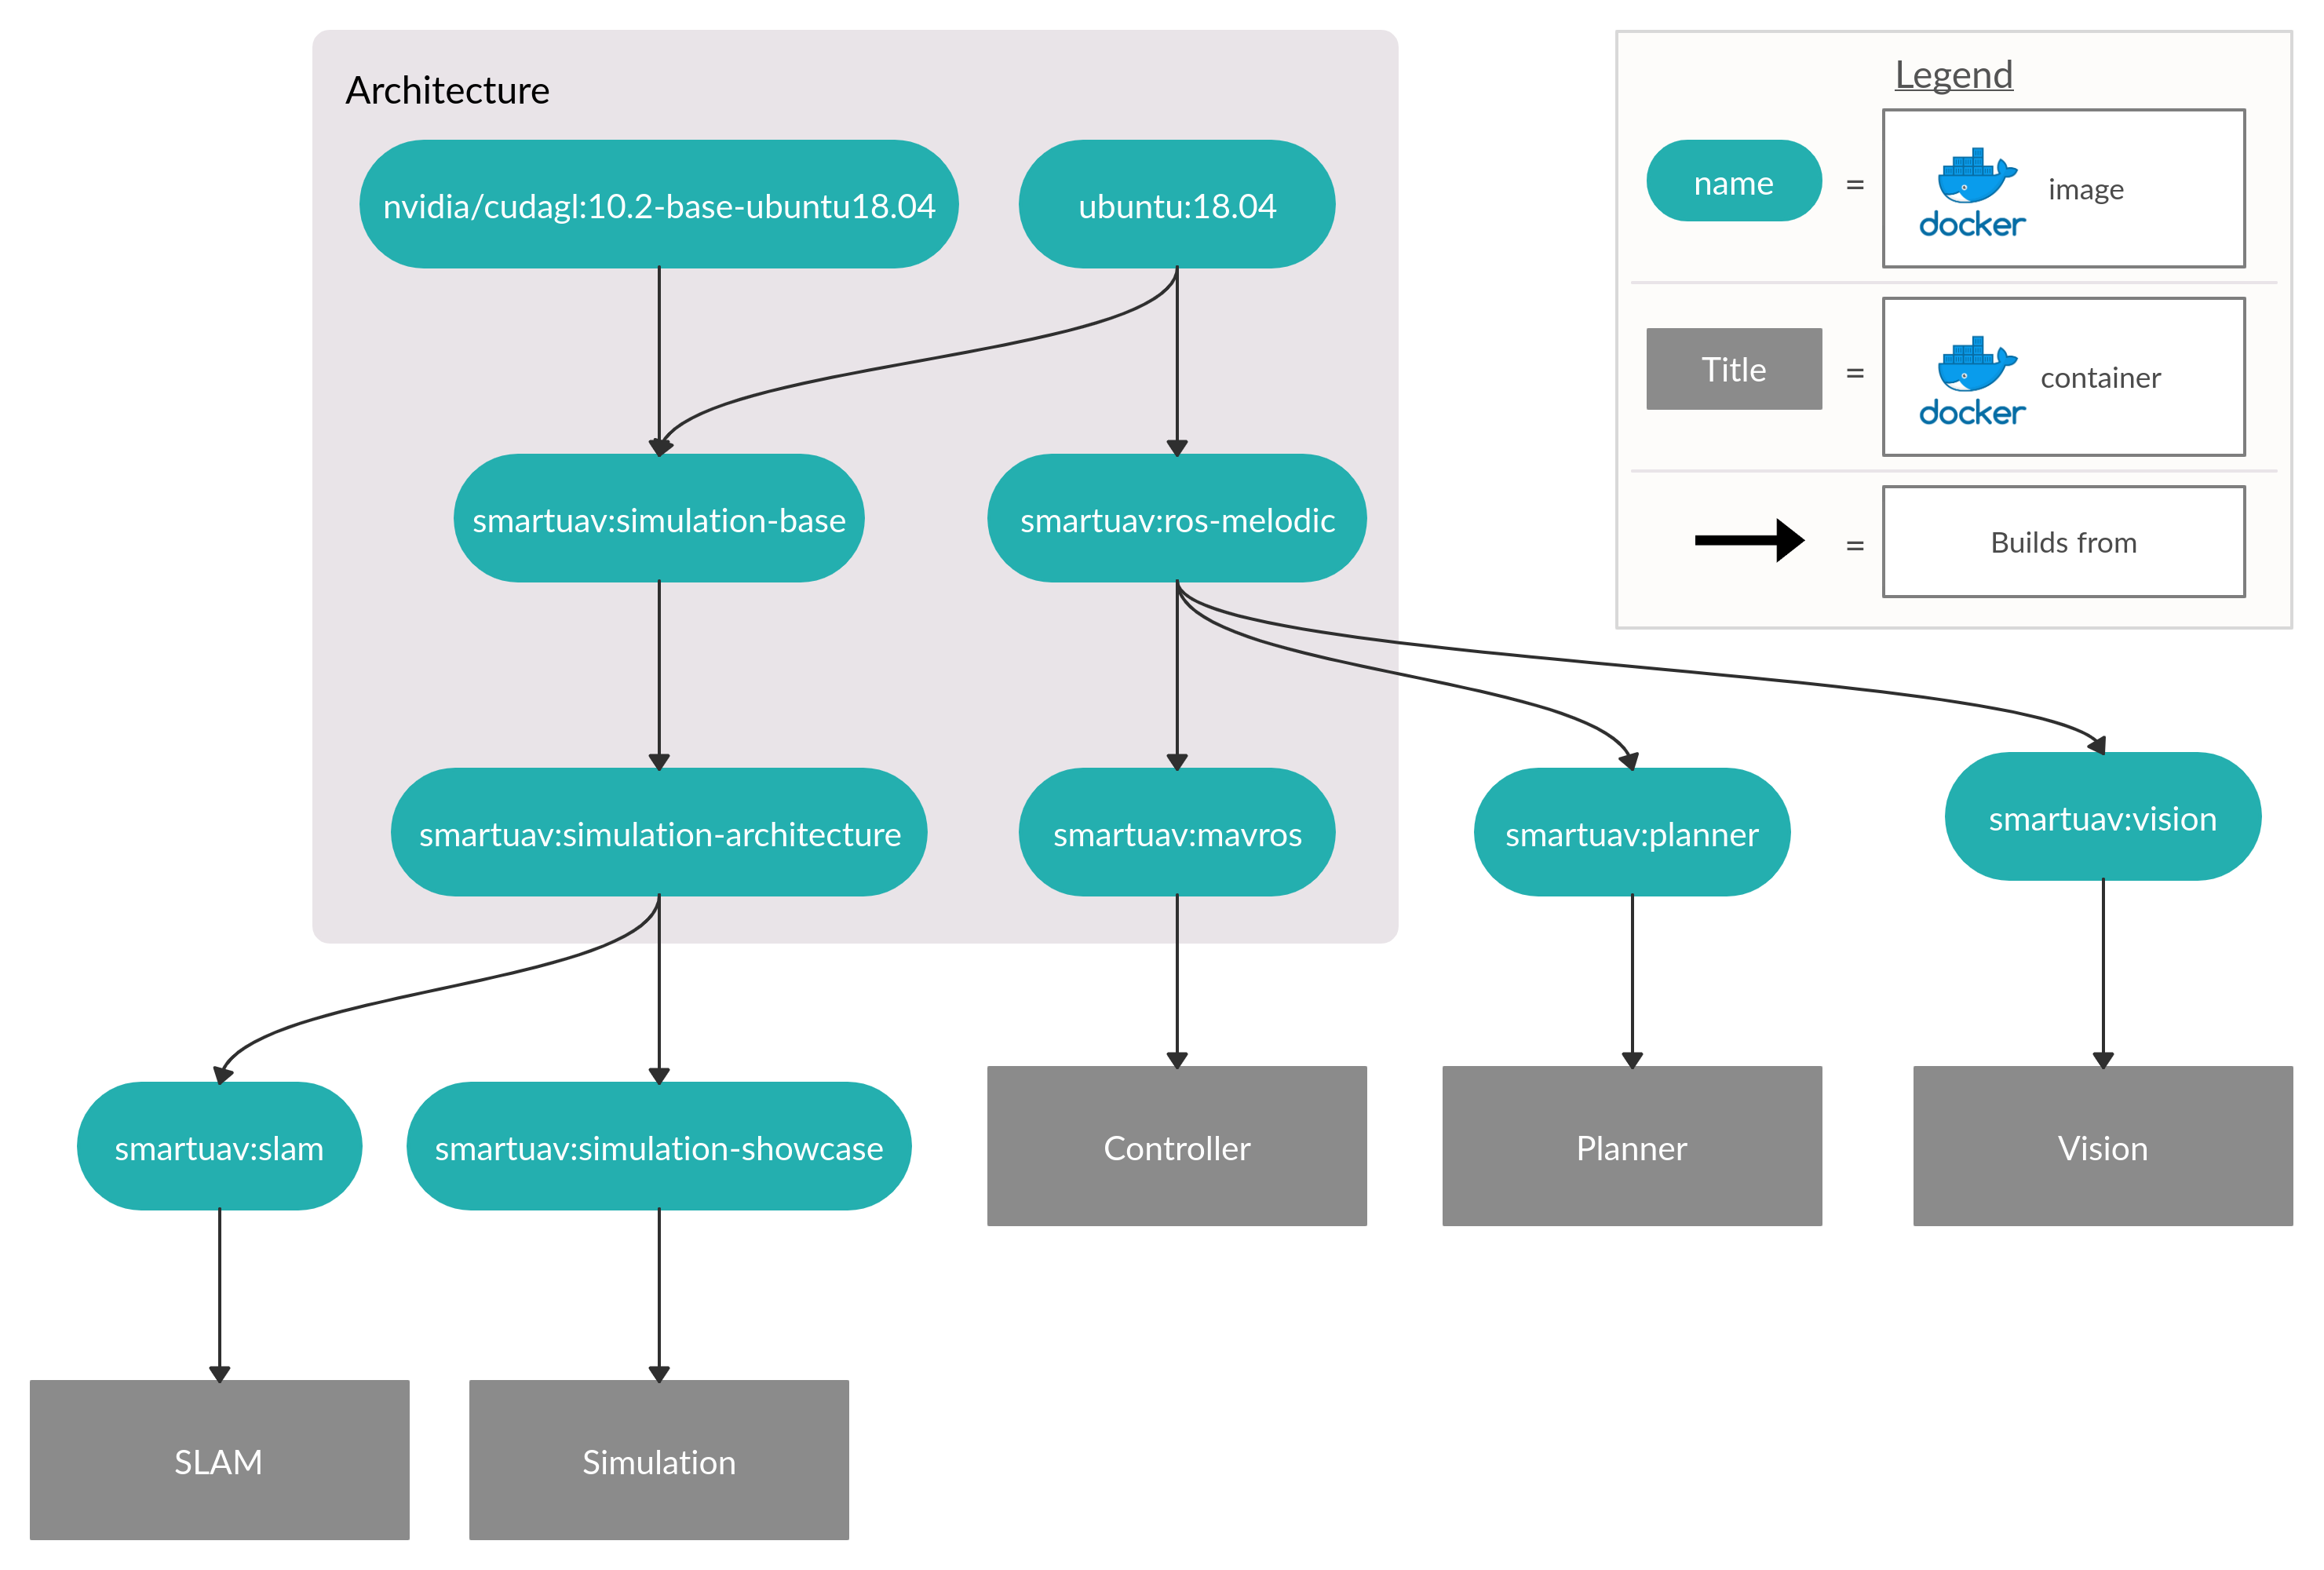
\includegraphics[width=\linewidth]{images/showcase_images.png}
  \caption{Docker images showcase}
\end{figure}

\clearpage

The showcase is used to conduct research, visualize this research, and show the capabilities of the architecture. Figure~\ref{fig:showcase_containers} visualizes which containers are run in the showcase and how there are connected.

\begin{figure}[!h]
  \centering
  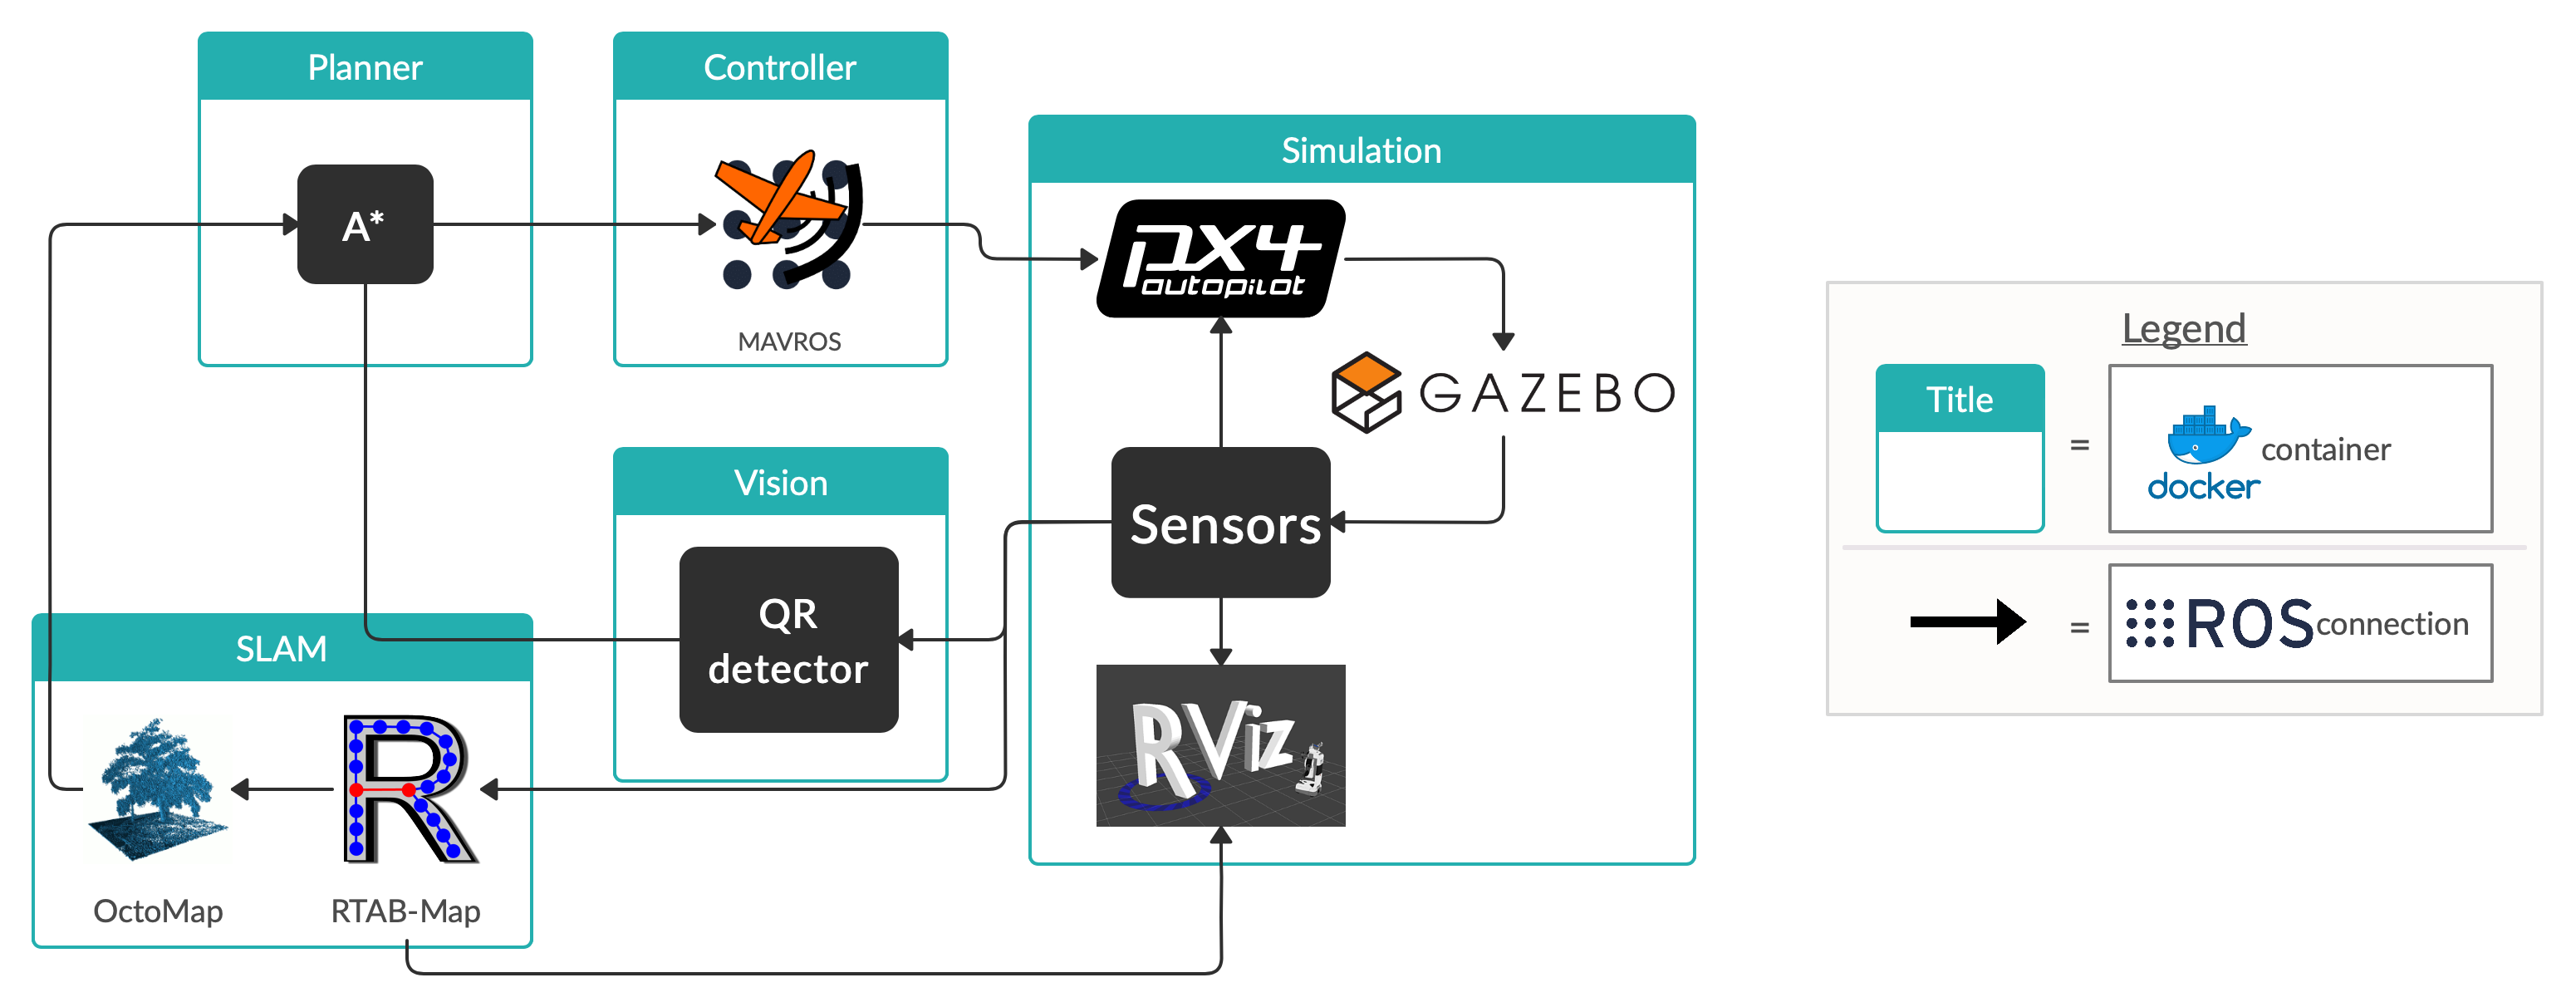
\includegraphics[width=\linewidth]{images/showcase_containers.png}
  \caption{Docker containers showcase}
  \label{fig:showcase_containers}
\end{figure}

  \chapter{Research topic}
  The research topic of this paper contains, the autonomous navigation of a \acs{uav} in a dynamic indoor environment. Since this topic encloses multiple aspects, it has been subdivided into multiple sub\hyp{}questions. They each answer a part of the research topic and are combined in the conclusion.

\begin{outline}
  \1 What defines a dynamic indoor environment?
    \2 What is the definition of a dynamic environment?
    \2 What is an indoor environment?
  \1 How is a \acs{uav} able to orientate in its environment?
    \2 How can a \acs{uav} observe its environment?
      \3 Wich sensors can a \acs{uav} use for observing its environment?
    \2 How is a \acs{uav} able to execute mapping and localization?
      \3 Which SLAM algorithms are eligible for a \acs{uav}?
  \1 How is a path of a \acs{uav} to a goal planned?
    \2 What defines an executable path?
    \2 How is the goal of a \acs{uav} defined?
    \2 Which path planning algorithms are usable?
  \1 How can a \acs{uav} execute a path?
  \1 What are the unsolved difficulties?
\end{outline}
  \clearpage
    \section{What defines a dynamic indoor environment?}
    The dynamic indoor environment created for the research is visualized in figure~\ref{fig:indoor_gazebo}. The environment is simulated in Gazebo. The definition of a dynamic environment and the properties of an indoor environment are noted in the following sections.

\begin{figure}[!h]
  \centering
  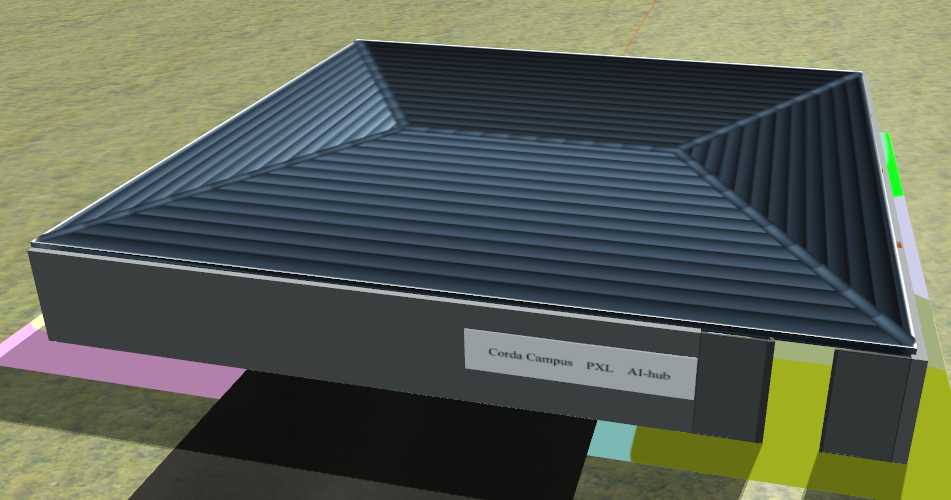
\includegraphics[width=0.6\linewidth]{images/indoor_environment_roof.png}
  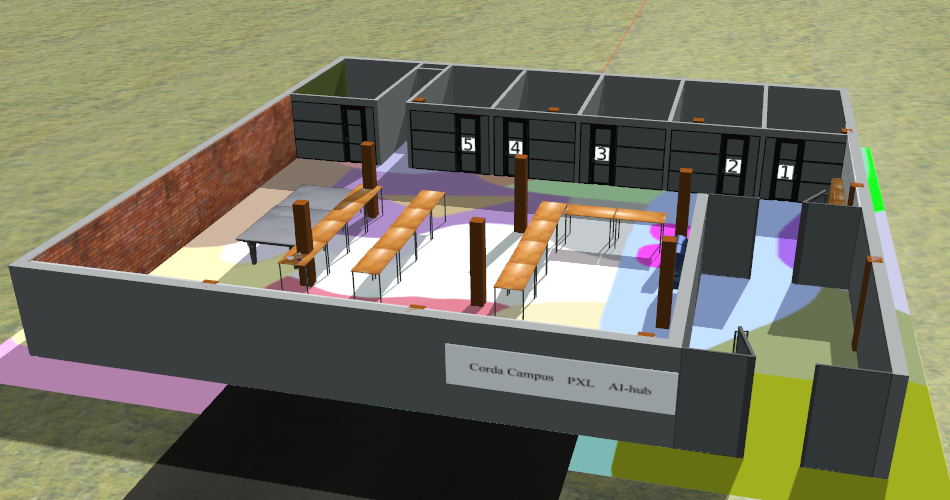
\includegraphics[width=0.6\linewidth]{images/indoor_environment_without_roof.png}
  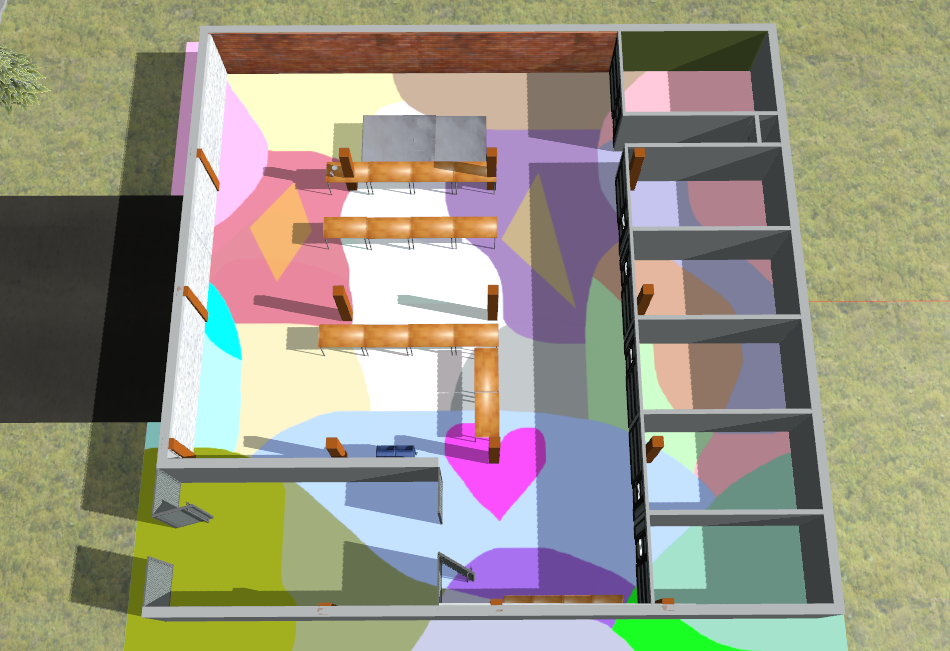
\includegraphics[width=0.6\linewidth]{images/indoor_environment_top.png}
  \caption{Environment simulated in Gazebo}
  \label{fig:indoor_gazebo}
\end{figure}
      \subsection{What is the definition of a dynamic environment?}
      To make an environment dynamic, it must have the ability to change over time. The change can be numerous things such as moving objects or persons, light intensity, and many other elements that can be detected by the sensors.
      \subsection{What is an indoor environment?}
      The main property of an indoor environment is that it is enclosed with walls, a ceiling, and a floor. An indoor environment is generally smaller than an outdoor environment. Therefore it is easier to map, but harder to navigate.

The easiest way for localization in an outdoor environment is the usage of a \acs{gps}. However, the \acs{gps} is not only blocked by the walls and ceiling of an indoor environment, but it is also not accurate enough for precise navigation.

\begin{table}[!h]
  \centering
  \begin{tabular}{| c | l |}
    \hline
    \textbf{Component} & \textbf{Implication}\\
    \hline
    \multirow{3}{*}{Enclosed} & Defined volume\\
    & Less or no \acs{gps} signal\\
    & Height limit\\
    \hline
    Lack of \acs{gps} & Not a reliable way to localize via \acs{gps}\\
    \hline
    Height limit & Harder to avoid object\\
    \hline
  \end{tabular}
  \caption{Indoor components}
\end{table}
      \clearpage
    \section{How is a UAV able to orientate in its environment?}
    Orientation in an environment can be obtained by first observing the environment, then mapping the observations, and finally locate the current location of the \acs{uav} in this map.
      \subsection{How can a UAV observe its environment?}
      The first action for orientation is observing the environment. This can be realized with sensors on the \acs{uav} that receive data related to its environment. There must also be accounted for dynamic properties.
      \clearpage
        \subsubsection{Which sensors can a UAV use for observing its environment?}
        A sensor is a piece of hardware mounted on the \acs{uav} that gathers data about the environment or itself is some way. A \acs{uav} has many sensors already attached to it, but there is a numerous amount of sensors that can be added. For example, different types of cameras or \acsp{lidar}. The sensors used in this project are picked by conducting research, using common sense, and by the requirements of the implemented \acs{slam} algorithm.

% http://breckon.eu/toby/publications/papers/magnabosco13slam.pdf
The most commonly used sensors for \acs{slam} algorithms are optical sensors. Optical sensors may be \acs{1d}, \acs{2d}, or \acs{3d} \acsp{lidar}, \acs{2d} or \acs{3d} sonar sensors, or a monocular, stereo or \acs{rgbd} camera. All sensors have their pros and cons, depicted in table~\ref{tab:sensors} \cite{slam_sensor_handover}

\begin{table}[!h]
  \centering
  \begin{tabular}{| c | c | c |}
    \hline
    \textbf{Sensor} & \textbf{Pros} & \textbf{Cons}\\
    \hline
    \acs{1d} \acs{lidar} & Low cost & Limited range of detection\\
    \hline
    \multirow{3}{*}{\acs{2d} \acs{lidar}} & Medium cost & \multirow{3}{*}{No vertical detection}\\
    & 360$^{\circ}$ detection &\\
    & Commonly used in \acs{slam} &\\
    \hline
    \acs{3d} \acs{lidar} & 360$^{\circ}$ detection on various angles & High cost\\
    \hline
    \multirow{3}{*}{Monocular camera} & \multirow{3}{*}{Cheap} & Minimal information\\
    & & Compute very heavy for depth\\
    & & Poor in low light\\
    \hline
    \multirow{3}{*}{Stereo camera} & Good in\hyp{}and outdoors & Compute heavy for depth\\
    & Low cost & Requires textures \\
    & Rich of information & Poor in low light \\
    \hline
    \multirow{2}{*}{\acs{rgbd} camera} & No ambient light needed & Poor oudoor performance\\
    & Compute unintensive for depth & Affected by reflection\\
    \hline
  \end{tabular}
  \caption{Pros and cons of sensors \cite{3d_camera}}
  \label{tab:sensors}
\end{table}
      \subsection{How is a UAV able to execute mapping and localization?}
      In this project, mapping and localization closely linked together. In order to create a map, the current location of the \acs{uav} in its area has to be known to be used as a reference point. However, to get the current location of the \acs{uav} in its area, the map of its area has to be known. Therefore, it can be described as a "chicken\hyp{}and\hyp{}the\hyp{}egg" problem.

% https://medium.com/desn325-emergentdesign/s-l-a-m-tech-tracking-743d059b1468
This issue can be overcome through the usage of a pre-existing map of an environment, for example, \acs{gps} data. However, there is no data for an indoor environment and if there was, it would not be precise enough or updated in real\hyp{}time. Therefore, the introduction of a \acs{slam} algorithm. This algorithm is capable of mapping and localization simultaneously with the usage of feature points.

% https://www.andreasjakl.com/basics-of-ar-slam-simultaneous-localization-and-mapping/
A \acs{slam} system is made up of four parts: sensor data, a front\hyp{}end, a back\hyp{}end, and the \acs{slam} estimate. The sensor data is all the input data a \acs{slam} system receives. In the front\hyp{}end a feature extraction process is executed. These features are tracked through a stream of video in the back\hyp{}end. The back\hyp{}end also handles long\hyp{}term associations to reduce drift and triggers loop\hyp{}closures. As a result, the \acs{slam} systems outputs all tracked features with their locations and relations, as well as the position of the sensors within the world.

% https://www.andreasjakl.com/basics-of-ar-anchors-keypoints-feature-detection/
As earlier mentioned, a \acs{slam} algorithm uses feature extraction as a way to track the movement of the \acs{uav} in space. The easiest way to explain how feature extraction works is its implementation on a camera. On every frame, features are detected. The way these features are detected differ from algorithm to algorithm. Every feature detected, needs a unique description based on its properties. 

The tracking of the features throughout the frames is handled in the back\hyp{}end. The descriptions of these features of different frames are compared. If most of the features change position in a certain way, the algorithm assumes the \acs{uav} has moved based on the change of position of features. The other features that do not changed position or in a different direction are considered as outliers or moving objects.

Not only the tracking of features is considered when estimating the motion of the \acs{uav}, but different sensor data influence the estimation. Most notable, the data from an accelerometer and a gyroscope. When the algorithm detects a frame it already has visited, it will recalculate all previous locations to match this new finding. This called a loop closure. With loop closures, a \acs{slam} algorithm keeps on updating previous values to keep the map as accurate as possible.
      \clearpage
        \subsubsection{Which SLAM algorithms are eligible for a UAV?}
        The decision of what \acs{slam} algorithms are eligible for use, depends on a couple of requirements stated by the project. The algorithm must output a \acs{3d} dense point cloud with pose estimation of the \acs{uav}. This pose estimation will be used for path planning later on. With these constraints in mind, a few algorithms were researched.
          \paragraph{ORB\hyp{}SLAM2}
          ORB\hyp{}SLAM2 is a real\hyp{}time \acs{slam} algorithm suitable for monocular, stereo and \acs{rgbd} cameras. It can handle loop closures and has relocalization capabilities. ORB-SLAM2 was developed in 2017 by Ra\'ul Mur\hyp{}Artal, Juan D. Tard\'os, J. M. M. Montiel, and Dorian G\'alvez\hyp{}L\'opez. The algorithm returns a sparse \acs{3d} reconstruction with true scale. \cite{orb_slam2_github} \cite{mur_orb_slam_2}

The algorithm has an option to compiled with \acs{ros}. Therefore it seemed a reasonable option for this project. After the implementation and some experimenting with ORB\hyp{}SLAM2, it became clear that the density of the point cloud was to sparse for this project.

\begin{figure}[!h]
  \centering
  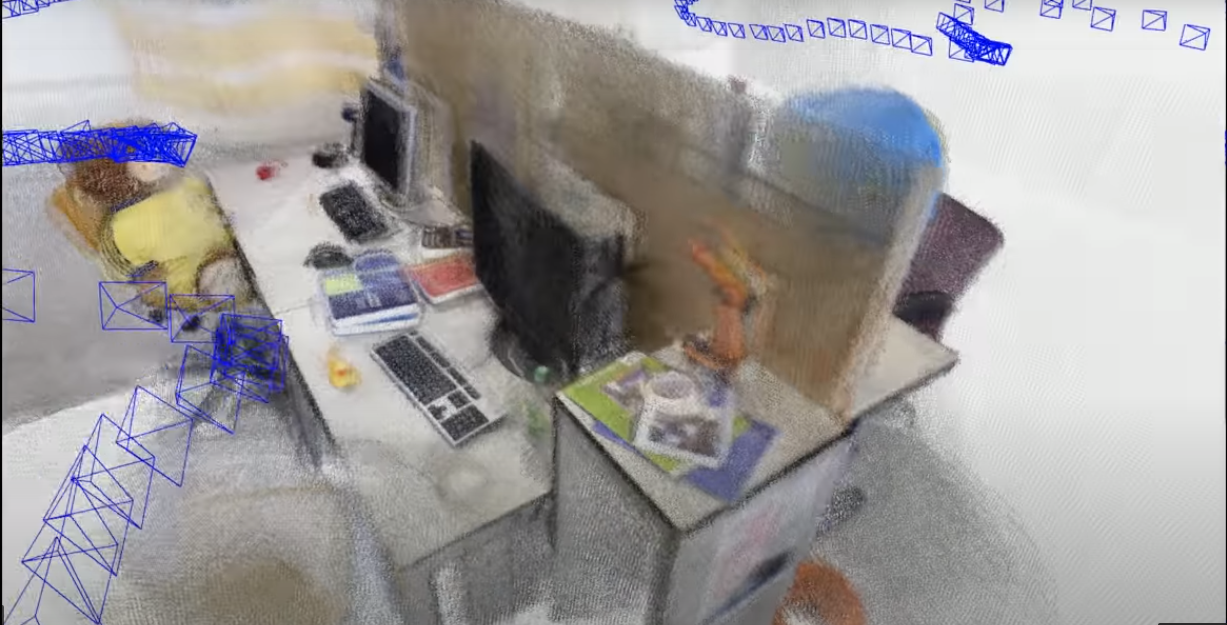
\includegraphics[width=\linewidth]{images/orb_slam2.png}
  \caption{ORB\hyp{}SLAM2 example \cite{orb_slam2_youtube}}
\end{figure}
          \clearpage
          \paragraph{Cartographer}
          % https://google-cartographer-ros.readthedocs.io/en/latest/
Cartographer is a real\hyp{}time \acs{slam} system that support \acs{2d} and \acs{3d} across multiple platforms and sensor configurations. Aswell as a build\hyp{}in \acs{ros} implementation. The system is developed and maintained by Google. \cite{cartographer_ros_integration}

% https://www.mdpi.com/2220-9964/5/11/212
The reason for researching this algorithm is that it is well maintained and often used in a lot of projects. The conclusion that Cartographer is not a real \acs{3d} but more a \acs{2.5d} algorithm came during the research. \acs{2.5d} is a pseudo\hyp{}\acs{3d} perspective. The algorithm can combine multiple \acs{2d} scans and combine them, but that is not truly \acs{3d}. \cite{liang2016generating}

\begin{figure}[!h]
  \centering
  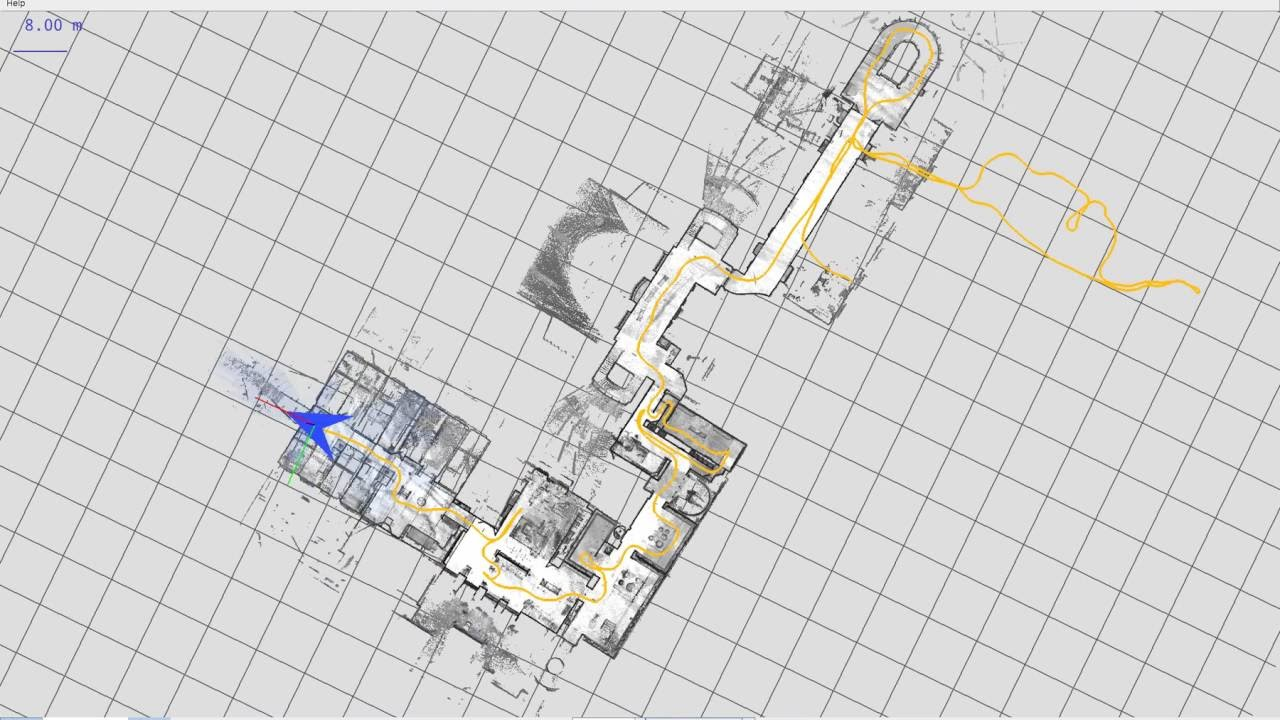
\includegraphics[width=0.75\linewidth]{images/cartographer_2d.jpg}
  \caption{Cartographer 2D example \cite{cartographer_google_open_source}}
\end{figure}

\begin{figure}[!h]
  \centering
  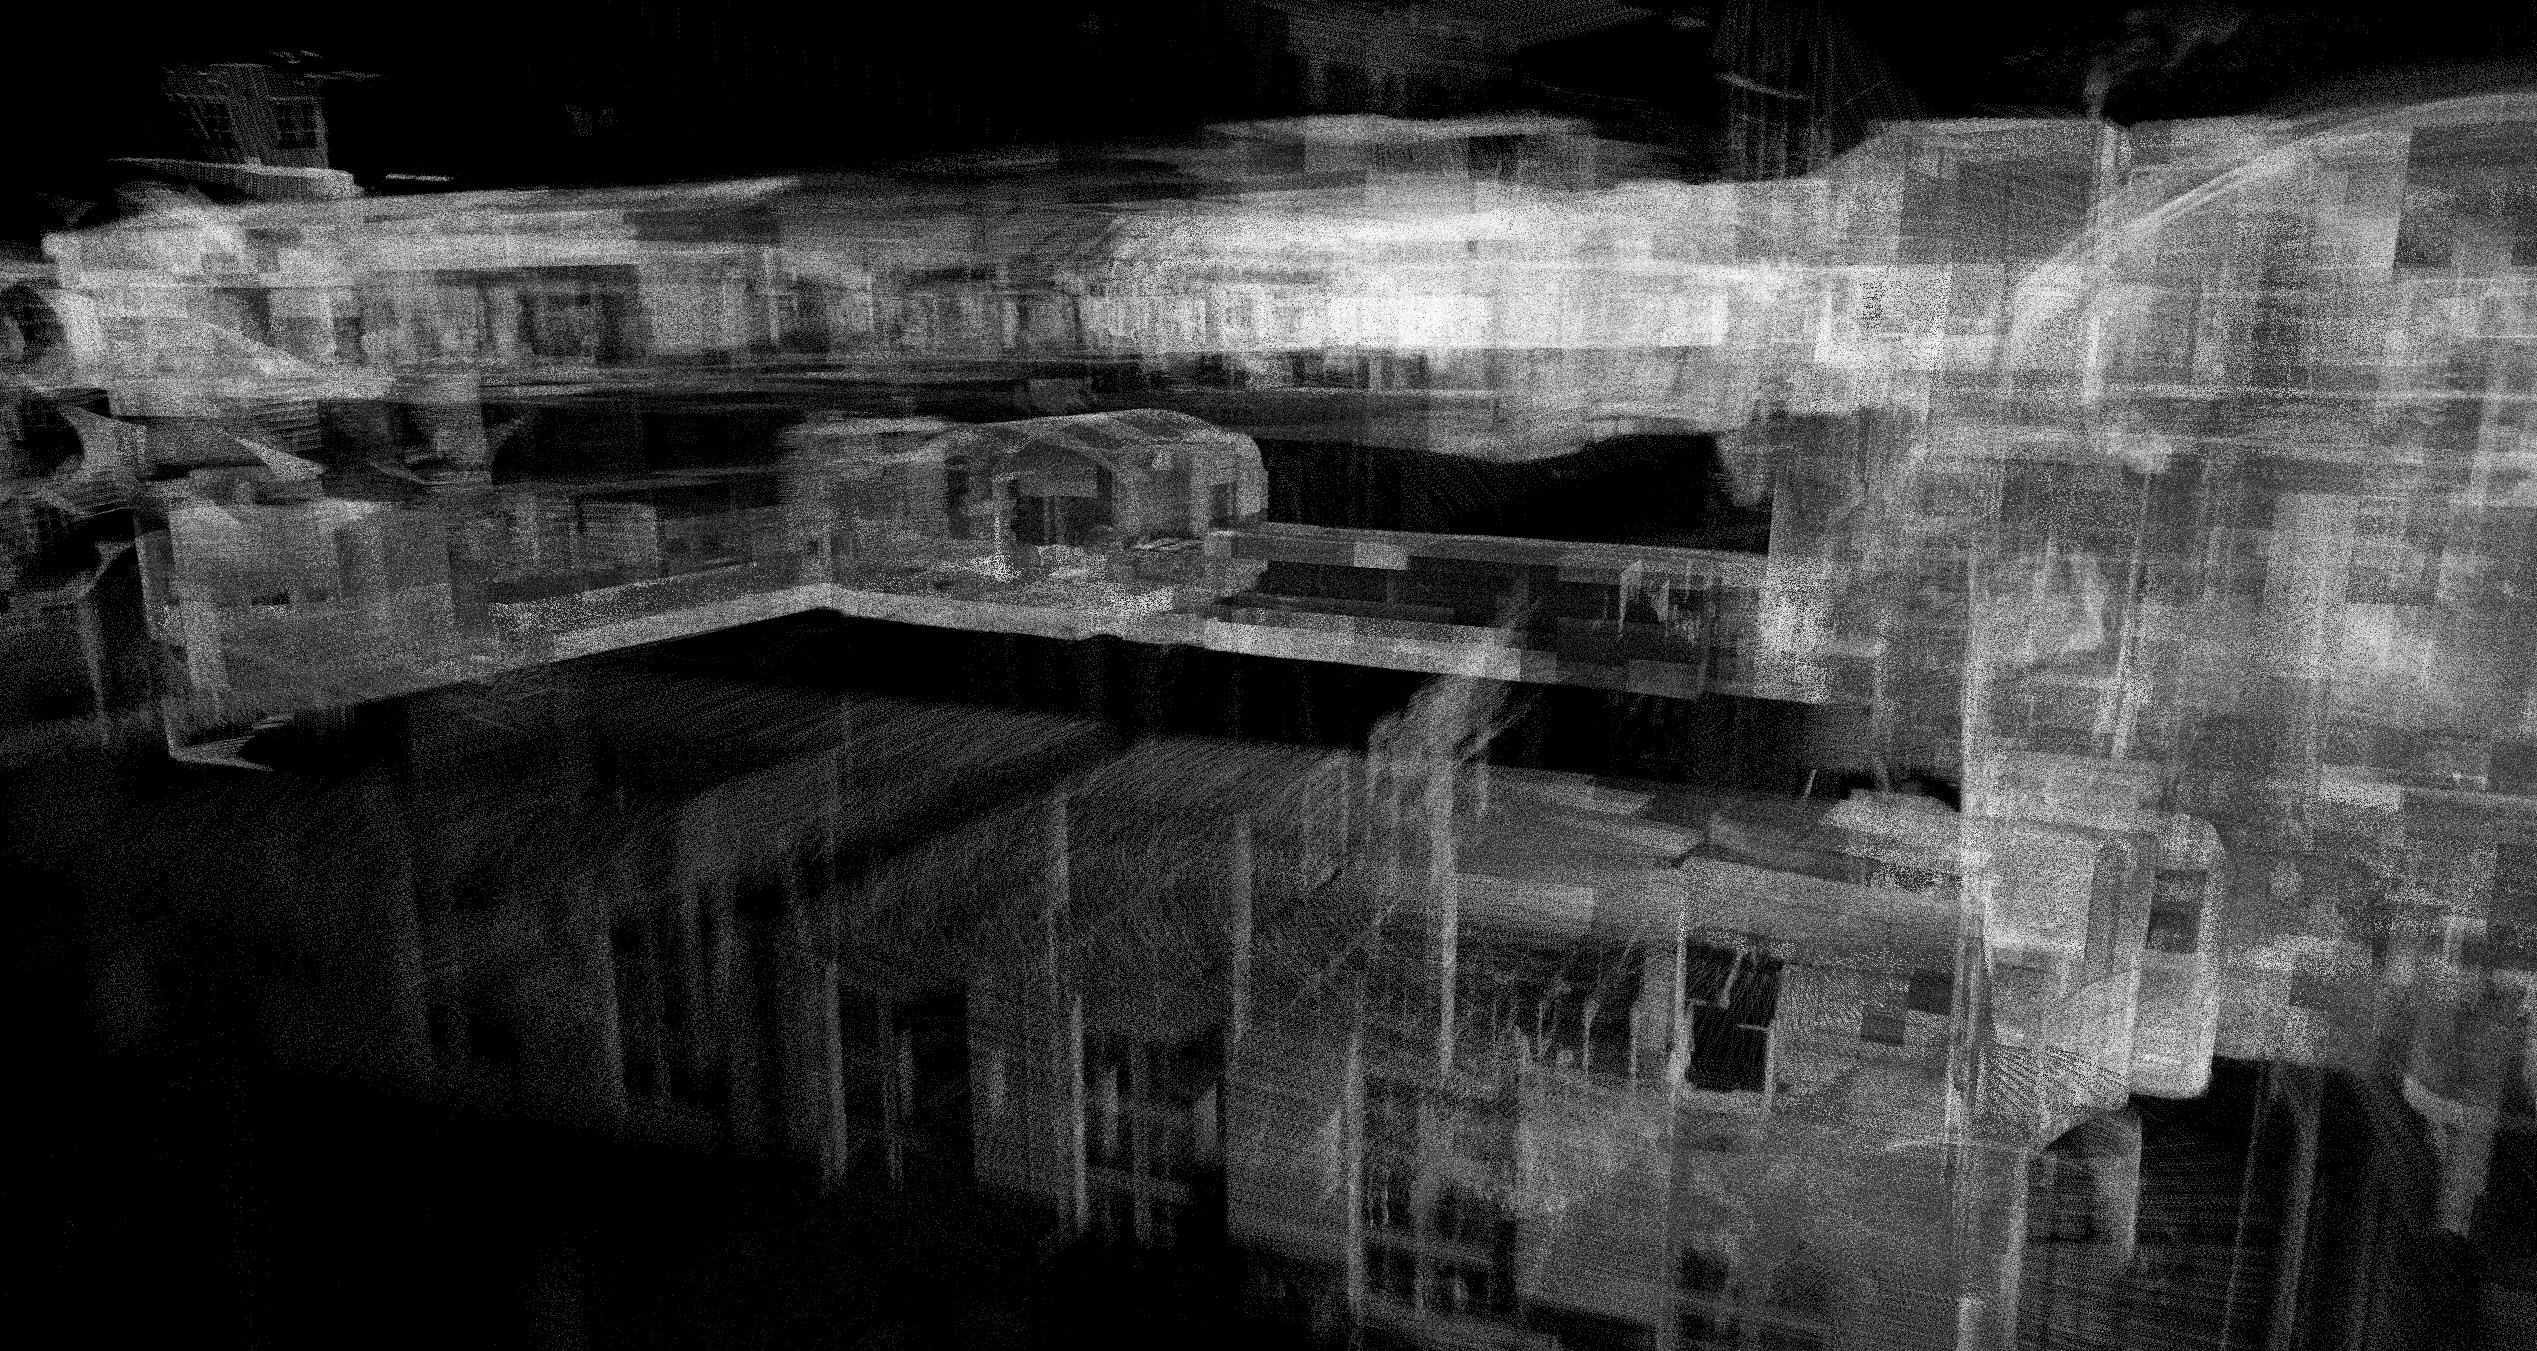
\includegraphics[width=0.75\linewidth]{images/cartographer_3d.jpg}
  \caption{Cartographer 3D example \cite{cartographer_exploiting_map}}
\end{figure}
          \paragraph{BLAM!}
          \acs{blam} is an open\hyp{}source \acs{lidar} based real\hyp{}time \acs{3d} \acs{slam} software package. Developed in 2016 by Erik Nelson from the \ac{bair} laboratory. The software is build in a \acs{ros} environment, containing two \acs{ros} workspaces. \cite{github_blam}

Because of its outdated dependencies and the difficulty of installation, there was no implementation possible of \acs{blam} in this project. \acs{blam} has \acs{ros}, \acs{gtsam}, and Boost as a dependency. The algorithm looked promising, but it does not support a camera as a sensor for visual odometry.

\begin{figure}[!h]
  \centering
  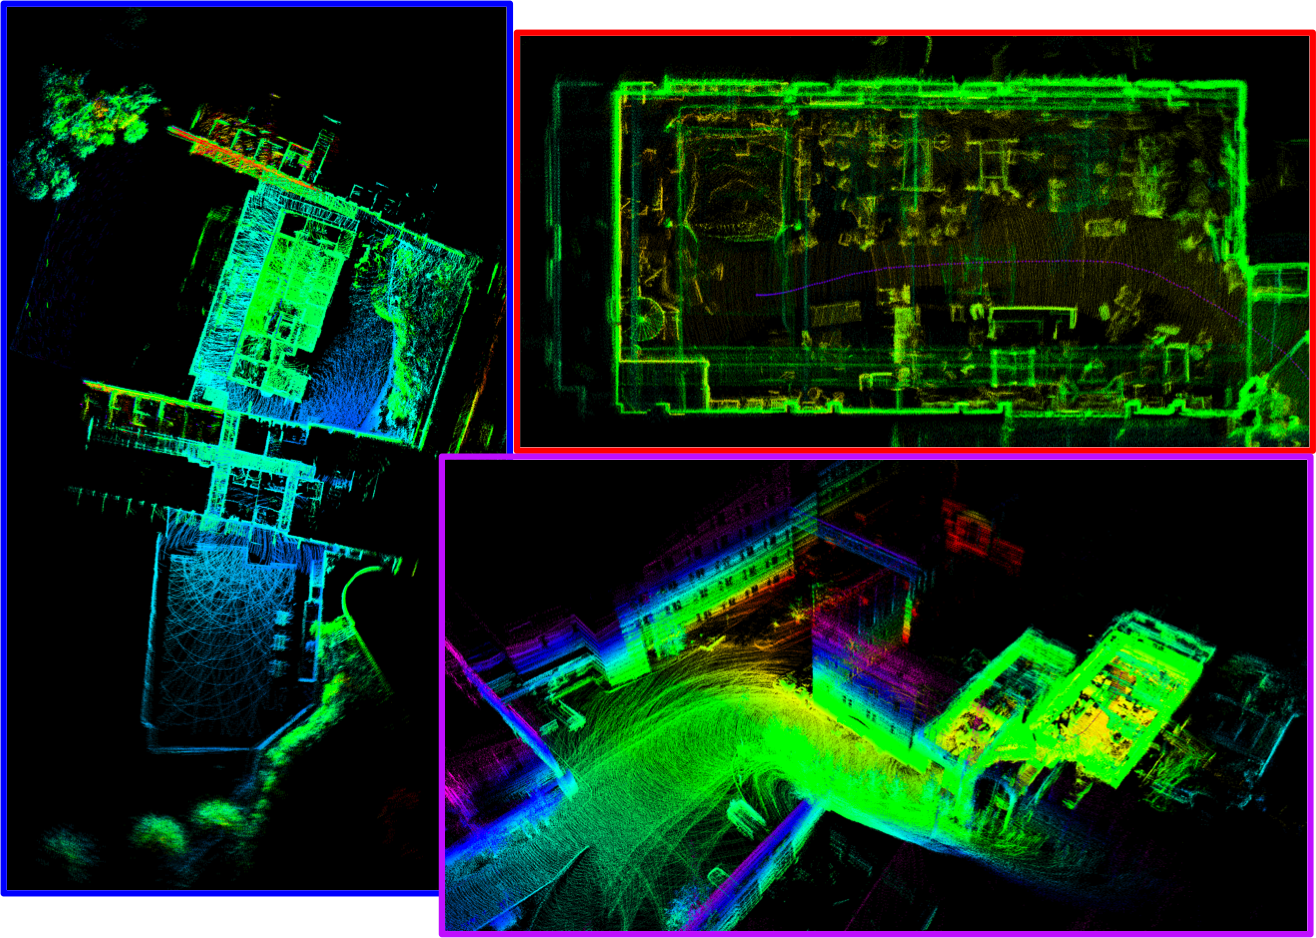
\includegraphics[width=\linewidth]{images/blam.png}
  \caption{BLAM! example \cite{github_blam}}
\end{figure}
          \clearpage
          \paragraph{hdl\_graph\_slam}
          % https://www.researchgate.net/publication/331283709_A_portable_three-dimensional_LIDAR-based_system_for_long-term_and_wide-area_people_behavior_measurement
The build in a \acs{ros} package \mbox{hdl\_graph\_slam} is an open\hyp{}source \acs{3d} \acs{lidar} based \acs{slam}. The package has been tested in indoor and outdoor environments with a Velodyne HDL\hyp{}32E, a Velodyne VLP\hyp{}16, and a RobotSense RS\hyp{}\acs{lidar}\hyp{}16. The package is developed in 2019 by Kenji Koide, Jun Miura, and Emanuele Menegatti. It supports multiple constraints that can be individually be enabled or disabled, being odometry, loop closure, \acs{gps}, \acs{imu} acceleration, \acs{imu} orientation, and floor plane detection. \cite{koide2019portable}

This package was the first fully implemented \acs{slam} algorithm of this project. Not being able to deal with loop closes was its mayor flaw for this project. It worked perfectly when not disturbed, therefore it was not reliable.

\begin{figure}[!h]
  \centering
  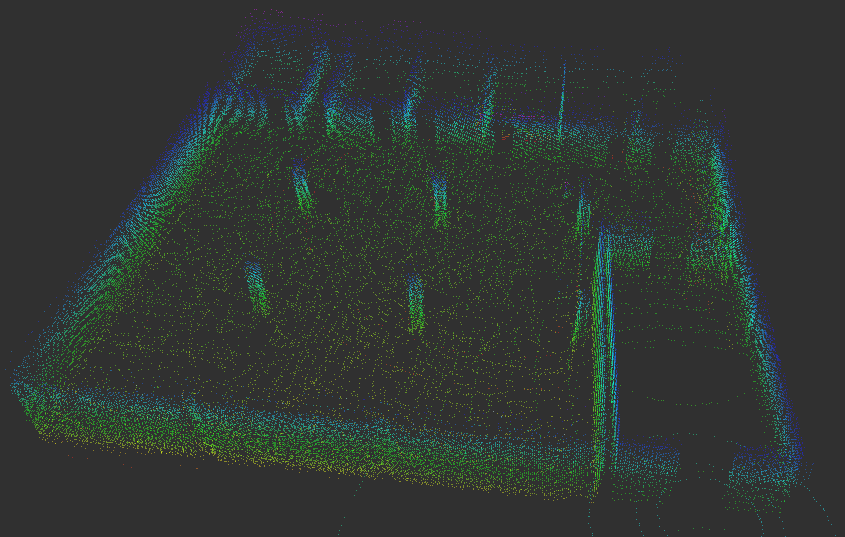
\includegraphics[width=\linewidth]{images/hdl_graph_slam_implementation.png}
  \caption{Implementation of hdl\_graph\_slam}
  \label{fig:hdl_graph_slam_implementation}
\end{figure}
          \clearpage
          \paragraph{RTAB\hyp{}Map}
          % http://introlab.github.io/rtabmap/
\acs{rtabmap} is an open\hyp{}source \acs{rgbd}, stereo camera and, \acs{lidar} graph\hyp{}based \acs{slam} system. The system is based on an incremental appearence\hyp{}based loop closure detector. The detector uses a bag\hyp{}of\hyp{}words approach to determine how likely a new image comes from a previous or a new location. \acs{rtabmap} is a standalone application available for Ubuntu, MacOSX, Windows, and a Raspberry Pi. But, also as a \acs{ros} package and on the Google Play Store. It is a heavily maintained piece of software. \cite{rtabmap_introlab}

The \acs{ros} package of \acs{rtabmap} has a lot of parameters to be adjusted to a specific need. The build\hyp{}in support with OctoMap allows it to be used for path planning. \acs{rtabmap} meets all the requirements needed for this project.

\begin{figure}[!h]
  \centering
  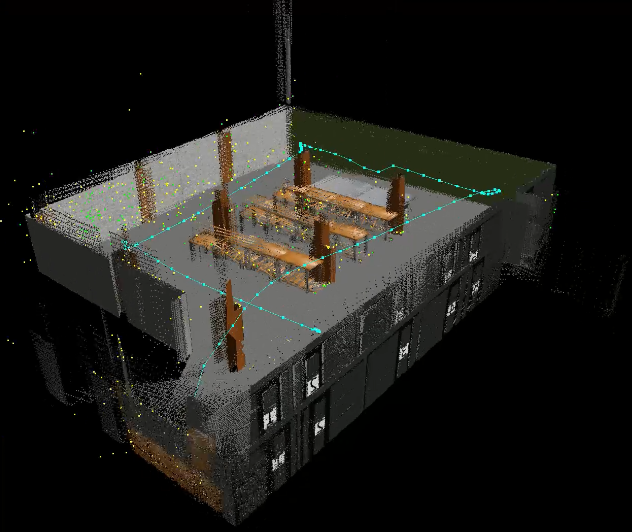
\includegraphics[width=0.7\linewidth]{rtabmap_implementation.png}
  \caption{Implementation of \acs{rtabmap}}
  \label{fig:rtabmap_implementation}
\end{figure}
          \clearpage
          \paragraph{Comparison SLAM algorithms}
          \begin{table}[!h]
  \centering
  \begin{tabular}{| c | c | c | c |}
    \hline
    \textbf{Algorithm} & \textbf{Sensors} & \textbf{Point cloud} & \textbf{Dimentional}\\
    \hline
    \multirow{3}{*}{ORB\hyp{}SLAM2} & Monocular camera & \multirow{3}{*}{sparse} & \multirow{3}{*}{\acs{3d}}\\
    & Stereo camera & &\\
    & \acs{rgbd} camera & &\\
    \hline
    Cartographer & Multiple configurations & dense & \acs{2d} \& \acs{3d}\\
    \hline
    \acs{blam} & \acs{3d} \acs{lidar} & dense & \acs{3d}\\
    \hline
    hdl\_graph\_slam & \acs{3d} \acs{lidar} & dense & \acs{3d}\\
    \hline
    \multirow{3}{*}{RTAB-Map} & Stereo camera & \multirow{3}{*}{dense} & \multirow{3}{*}{\acs{3d}}\\
    & \acs{rgbd} camera & &\\
    & \acs{3d} \acs{lidar} & &\\
    \hline
  \end{tabular}
  \caption{Comparison \acs{slam} algorithms}
\end{table}
          \clearpage
    \section{How is a path of a UAV to a goal planned?}
    % https://www.sciencedirect.com/book/9780128042045/wheeled-mobile-robotics
Path planning is the task of finding a continuous path from the start to the goal. The path planning algorithm must have a definiton of an executable path and a goal. The start is stated by the current position of the \acs{uav}. The algorithm receives a occupancy grid and returns the shortest path from start to goal. \cite{KLANCAR2017161}

% https://www.gamedev.net/tutorials/programming/general-and-gameplay-programming/introduction-to-octrees-r3529/
The occupancy grid is obtained as the output of \acs{rtabmap} and is represented in an Octree format. An Octree is a special type of subdividing tree in a \acs{3d} space. One node in an Octree can be subdivided into eight smaller nodes, each node represents a free or occupied space. \cite{octrees_gamedev}

\begin{figure}[!h]
  \centering
  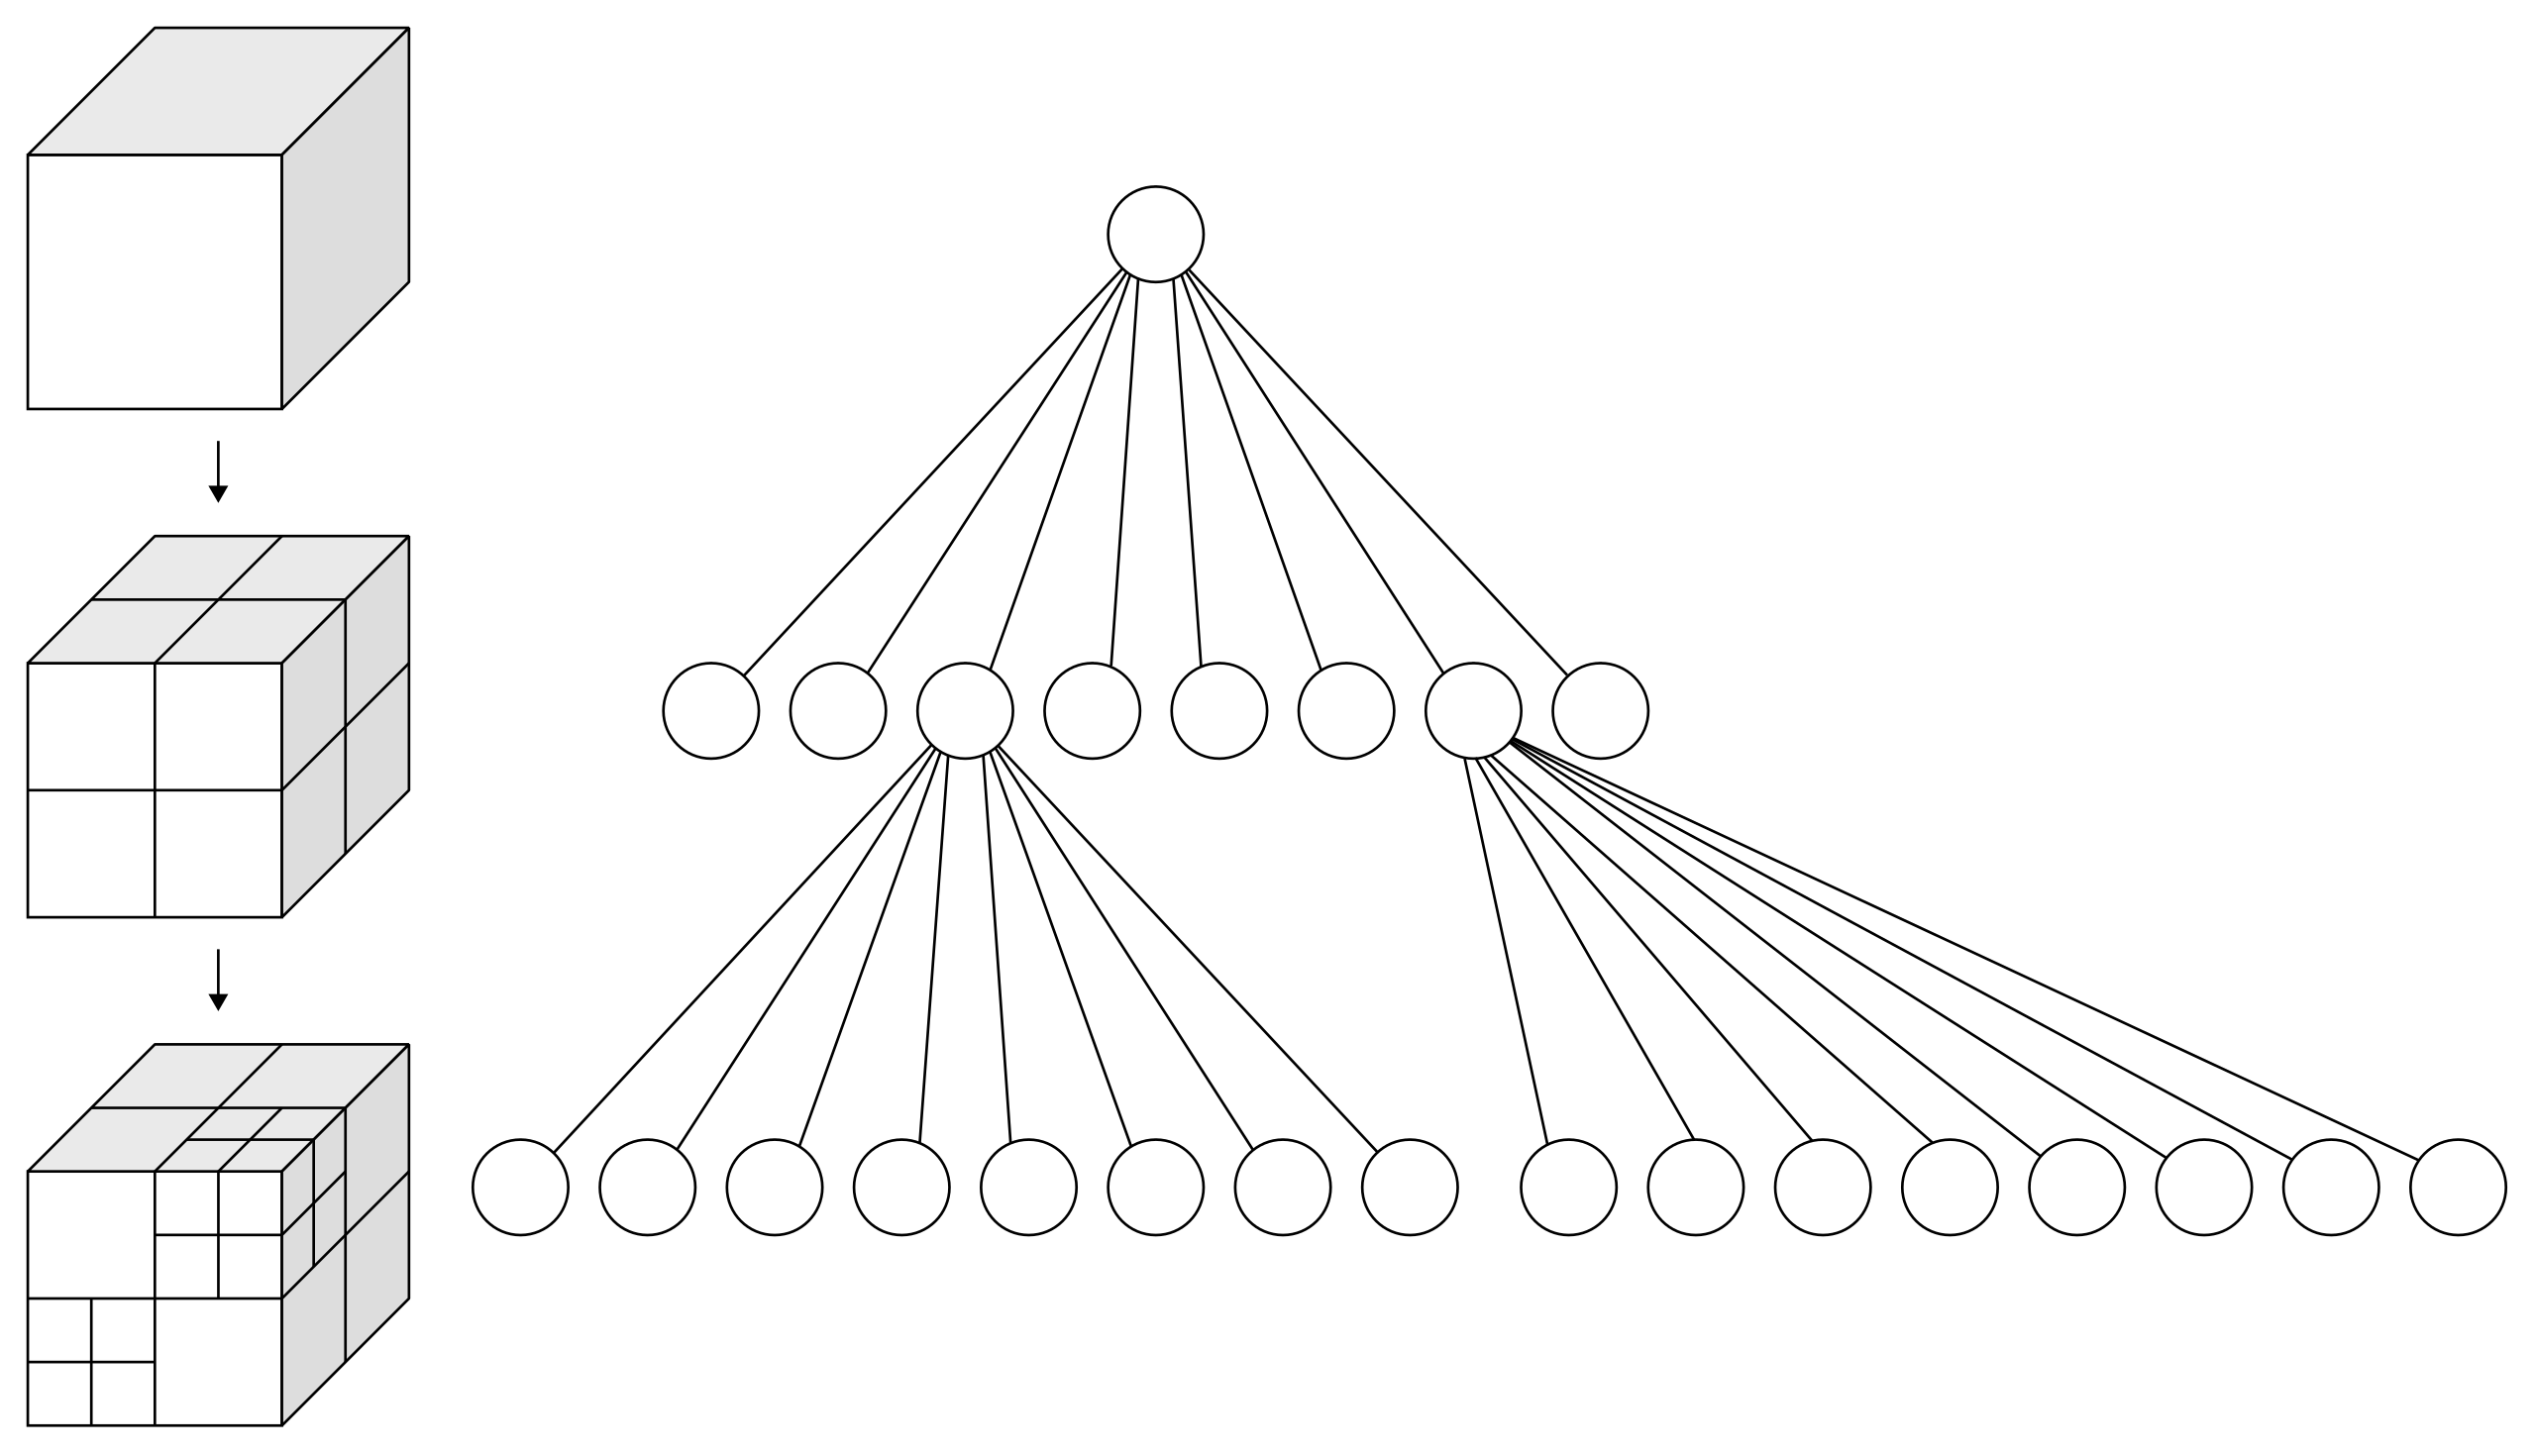
\includegraphics[width=0.6\linewidth]{images/octree.png}
  \caption{Octree \cite{octrees_gamedev}}
\end{figure}
      \subsection{What defines an executable path?}
      An executable path is defined as a path that the \acs{uav} can traverse. In other words, the path must be free of obstacles and account for the size of the \acs{uav} with an added margin. Because of the indoor environment, the path of the \acs{uav} must be precise and realistic. Therefore, the path should not be too close to walls, under tables, through cabinets, or other risks. At last, the path preferably should be as smooth as possible. The perfect path is the shortest path that meets all of the listed requirements.
      \clearpage
      \subsection{How is the goal of a UAV defined?}
      The goal is defined by a \acs{qrcode} placed in the world. One \acs{uav} explores the indoor environment searching for the \acs{qrcode}. Once found, another \acs{uav} plans a path with the \acs{qrcode} as its goal.

The \acs{qrcode} is generated with a repository that outputs a model for Gazebo with an image as input. The \acs{uav} can detect this code with the use of a \acs{ros} package. Once a \acs{qrcode} is detected, a message is published with its location for path planning. \cite{github_ar_tags_gazebo} \cite{github_qr_detector}
      \subsection{Which path planning algorithms are usable?}
      Because of time constraints in this project, the initial explore algorithm was not an option, this will be further explained in the section that describes the unsolved difficulties. Therefore, another approach was taken for the investigation. One \acs{uav} would first map the area and find the goal. In this mapped area, an optimal path is searched from the position of second \acs{uav} to the goal.

There are many path planning algorithms out there, but again because of the time constrains, only a few are researched. The main requirements are that it must be easily implementable in Python, can handle \acs{3d} and is flexible to add constraints such as the size of the \acs{uav}.
        \subsubsection{Dijkstra}
        % https://amturing.acm.org/award_winners/dijkstra_1053701.cfm
Dijkstra's algorithm is one of the most famous algorithms for finding the shortest path between nodes in a graph. The algorithm was published by Edsger W. Dijkstra in 1959. Not only having the option to return the shortest path, Dijkstra's algorithm can give the sortest path from the start to every other node.
        \clearpage
        \subsubsection{Lazy Theta*}
        Lazy Theta* is a path planning algorithm that can handle continuous \acs{2d} and \acs{3d} grid environments. It is built upon Theta* and uses lazy evaluation to improve the performance of the algorithm. \cite{lazy_theta_star}

The algorithm is a valid candidate for this project because it meets almost all the requirements. The only requirement it does not meet is the easy implementation in Python. Therefore, the search for another algorithm continued.
        \subsubsection{A*}
        A* is a popular and efficient search algorithm used in many fields of computer science. The algorithms is an extension of Dijkstra's algorithm with characteristics of breath-first search and the enhancement of heuristics. \cite{a_star_brilliant}

Different methods of calculating the distance between nodes can be used as a heuristic. Two of those methods are the Manhattan distance and the Euclidian distance. After the experimentation of both, the Euclidian was computationally heavier but resulted a more realistic path.

The algorithm is very flexible and easy to implement in Python. It can handle a 3D environment and account for the size of the \acs{uav} with minimal modifications. That is why A* is used in this project to get the shortest executable path from the position of the second \acs{uav} to the \acs{qrcode}.
        \clearpage
    \section{How can a UAV execute a path?}
    Once a valid path is obtained through path planning, it has to be executed by a \acs{uav}. The path is an array of coordinates. Once the \acs{uav} has reached a coordinate, it receives the next coordinate in the array until the goal is reached. The \acs{uav} reaches a coordinate when its current position is within a certain distance of the coordinate. This value is calculated with the euclidean distance.

The optimize the path, only the coordinates that go to a new direction in any axis are kept. If for example a sequence of coordinates have the same increment in x values and have the same y and z values, the only coordinates that contain useful information are the first and the last.

In figure~\ref{fig:path} the exectuable path is visualized. The red blocks are all the coordinates that are returned from the path planning algorithm, where the yellow blocks are the only points with useful information.

\begin{figure}[!h]
  \centering
  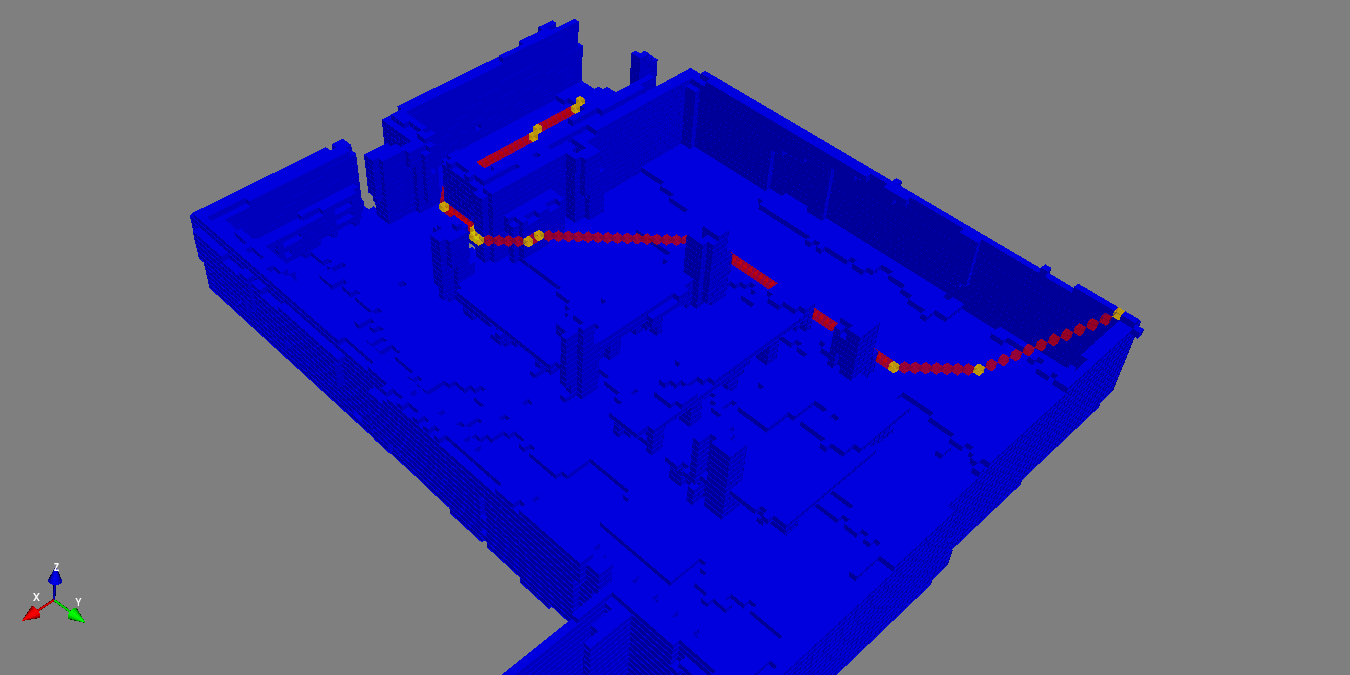
\includegraphics[width=\linewidth]{images/path.png}
  \caption{Executable path example}
  \label{fig:path}
\end{figure}
    \clearpage
    \section{What are the unsolved difficulties?}
    The developed system is not completely autonomous, the first \acs{uav} has to fly to the \acs{qrcode} manually for the second \acs{uav} to fly to this without any other input than the location of the goal and the mapped environment.

There is currently no \acs{ros} algorithm for exploration in a \acs{3d} environment. Because of time constraints and lack of expertise, writing such an algorithm based on a \acs{2d} implementation is not realistic. The performance of Python is not adequate to run such an algorithm in real time, a language such as C++ should be used for this.

The path planning or exploration algorithm should be executed directly on the Octree output of \acs{rtabmap}. However, in this project the Octree is converted to a \acs{3d} matrix to find the neighboring coordinates, which is an unnecessary conversion.

Because of developing in an simulated environment, the \acs{slam} algorithm detected loopclosures where they should not be detected. The simulated environment is created with textures that repeat and are exactly the same each time, in a real environment two exactly the same textures do not exist. To overcome this issue, an un realistic floor design was created that was streched over the whole surface. A better solution would be to create a better simulated environment with custom textures or add random noise to each texture.

  \nonumchapter{Conclusion}
  This project made it possible for many developers to develop \acs{uav} applications without much trouble setting up a developement environment. This is achieved by the created architecture, which is practically a finish product.

On the other hand the showcase is far from a finished product, but has made it clear where further research and development is needed. The research in this project has made it clear that currently \acs{2d} autonomous navigation is reasonably evolved, but the \acs{3d} aspect is still in its infancy.
  \nonumchapter{Bibliographical references}
  \printbibliography[heading=none]
\end{document}